% Chapter Template

\chapter{Triple Quantum Dot} % Main chapter title

\label{sec:TQD} % Change X to a consecutive number; for referencing this chapter elsewhere, use \ref{ChapterX}

%----------------------------------------------------------------------------------------
%	SECTION 1
%----------------------------------------------------------------------------------------

In this chapter we will focus on the study of a GaAs linear triple quantum dot (TQD) array populated with one heavy hole (HH).
\section{Hamiltonian and dark state}
Using Eq.~(\ref{eq:total_Hamiltonian}) we can write the Hamiltonian in the second quantization formalism as
\begin{equation}
	\begin{split}
	\hat{\mathcal{H}}_{\text{TQD}}=&\sum_i\varepsilon_i\hat{n}_i+\frac{1}{2}E_Z\sum_i(\hat{n}_{i\uparrow}-\hat{{n}_{i\downarrow}})-\sum_{\sigma}(t_{N,12}\hat{c}_{1\sigma}^\dagger \hat{c}_{2\sigma}+t_{N23}\hat{c}_{2\sigma}^\dagger \hat{c}_{3\sigma} + \text{H.c.})\\
	&-\sum_{\sigma\neq \sigma'}(t_{F,12}e^{i\theta_{12}}\hat{c}_{1\sigma}^\dagger \hat{c}_{2\sigma'}+t_{F,23}e^{i\theta_{23}}\hat{c}_{2\sigma}^\dagger \hat{c}_{3\sigma'}+\text{H.c.})\; ,
	\end{split}
\end{equation}
where the indices $i=1,2,3$ denote the left, center and right dot respectively. For simplicity we will set the phase of the spin-flip tunneling equal for each pair of QDs, so $\theta_{12}=\theta_{23}=\theta$. In this chapter we will work with the case in which all the dots are in resonance $\varepsilon_i=0$, and in absence of magnetic field $E_Z=0$, so the Hamiltonian is
\begin{equation}
	\hat{\mathcal{H}}_{\text{TQD}}=\mqty(0 & 0 & -t_{N,12} & -e^{i\theta}t_{F,12} & 0 & 0 \\
	0 & 0 & -e^{i\theta}t_{F,12} & -t_{N,12} & 0 & 0 \\
	-t_{N,12} & -e^{-i\theta}t_{F,12} & 0 & 0 & -t_{N,23} & -e^{i\theta}t_{F,23}\\
	-e^{-i\theta}t_{F,12} & -t_{N,12} & 0 & 0 & -e^{i\theta}t_{F,23} & -t_{N,23}\\
	0 & 0 & -t_{N,23} & -e^{-i\theta}t_{F,23} & 0 & 0 \\
	0 & 0 & -e^{-i\theta}t_{F,23} & -t_{N,23} & 0 & 0)\; .
\end{equation}
Our aim in this chapter is a long transference of the HH from one end of the QD array to the other, with the minimum population of the middle site as possible. For this we need to find if the system presents a dark state that populate both edges and with no weight in the middle dot. Solving the eigenvectors of the above Hamiltonian we obtain one possible dark state given by
\begin{equation}
	\begin{split}
	\ket{\phi_{\text{DS},1}}=\mathcal{N}&\left[\frac{e^{i\theta}t_{F,23}t_{N,12}-e^{-i\theta}t_{F,12}t_{N,23}}{-t_{N,12}^2+e^{-2i\theta}t_{F,12}^2}\ket{\uparrow,0,0}\right.\\
	&\;\left.+\frac{t_{F,12}t_{F,23}-t_{N,12}t_{N,23}}{t_{N,12}^2-e^{-2i\theta}t_{F,12}^2}\ket{\downarrow,0,0}+\ket{0,0,\downarrow}\right]\;
\end{split}
\end{equation}
where $\mathcal{N}$ is the normalization factor. The other dark state $\ket{\phi_{\text{DS},2}}$ is similar to this one under the interchange of the spin projections, so we will work just with the above state. Setting the spin-conserving and spin-flip tunnellings to be proportional $t_{F,ij}=xt_{N,ij}$ the dark state is now written as
\begin{equation}
	\begin{split}
	\ket{\phi_{\text{DS},1}}=\mathcal{N}&\left[\frac{t_{N,23}}{t_{N,12}(1-e^{-2i\theta}x^2)}\left(-2ix\ket{\uparrow,0,0}+(x^2-1)\sin(\theta)\ket{\downarrow,0,0}\right)+\ket{0,0,\downarrow}\right]\;.
	\label{eq:dark_state}
	\end{split}
\end{equation}
At this point we have two possibilities, we can have a long range transfer from the left dot to the right dot with and without spin-flip, depending on the parameters that we set. Let us study each case separately.

\section{Long range transference flipping spin}
Setting $x=1$ in Eq.~(\ref{eq:dark_state}) we obtain a dark state that connects both ends of the array with opposite spin in each edge
\begin{equation}
\ket{\phi_{\text{DS},1}}=-e^{i\theta}\cos(\varphi)\ket{\uparrow,0,0}+\sin(\varphi)\ket{0,0,\downarrow}\; ,
\end{equation} 
where we have defined the angle $\tan(\varphi)\equiv t_{N,12}/t_{N,23}$. At this point we can try to implement the CTAP protocol using Gaussian shape pulses for the tunneling rates
\begin{equation}
\begin{split}
t_{N,12}=t_0\exp[-\frac{(t-t_f/2+\tau_{12})^2}{\sigma^2}]\; ,\\
t_{N,23}=t_0\exp[-\frac{(t-t_f/2+\tau_{23})^2}{\sigma^2}]\; ,
\end{split}
\end{equation}
where we have introduced to parameters $\tau_{12}$ and $\tau_{23}$ to shift the pulses over time. Our aim is to transfer the hole from the left dot to the right dot, so it is intuitive to think that we must increase first the tunneling $t_{N,12}$ and later $t_{N,23}$, what is known as the intuitive order $\tau_{12}>\tau_{23}$. The result for the evolution of the system applying this ordering with $\tau_{12}=-\tau_{23}=\tau$ and $\sigma=\tau=t_f/6$ is shown in Fig.~\ref{fig:CTAP_TQD_Results} b). We can however apply the counter-intuitive order in which the tunneling between the center and right dots is increased before than the tunneling between the left and center dots. Setting $\tau_{N,12}=-\tau_{N,23}=-\tau$ now we obtain a different evolution for the states, Fig.~\ref{fig:CTAP_TQD_Results} d). We can clearly see that the best result is obtained with the counter-intuitive order, something that is already known in the literature \cite{Greentree2004}. However, the fidelity hardly reaches a value of $\mathcal{F}=0.75$, in addition to the fact that the population of the middle states is not negligible.
\begin{figure}[!htb]
	\centering
	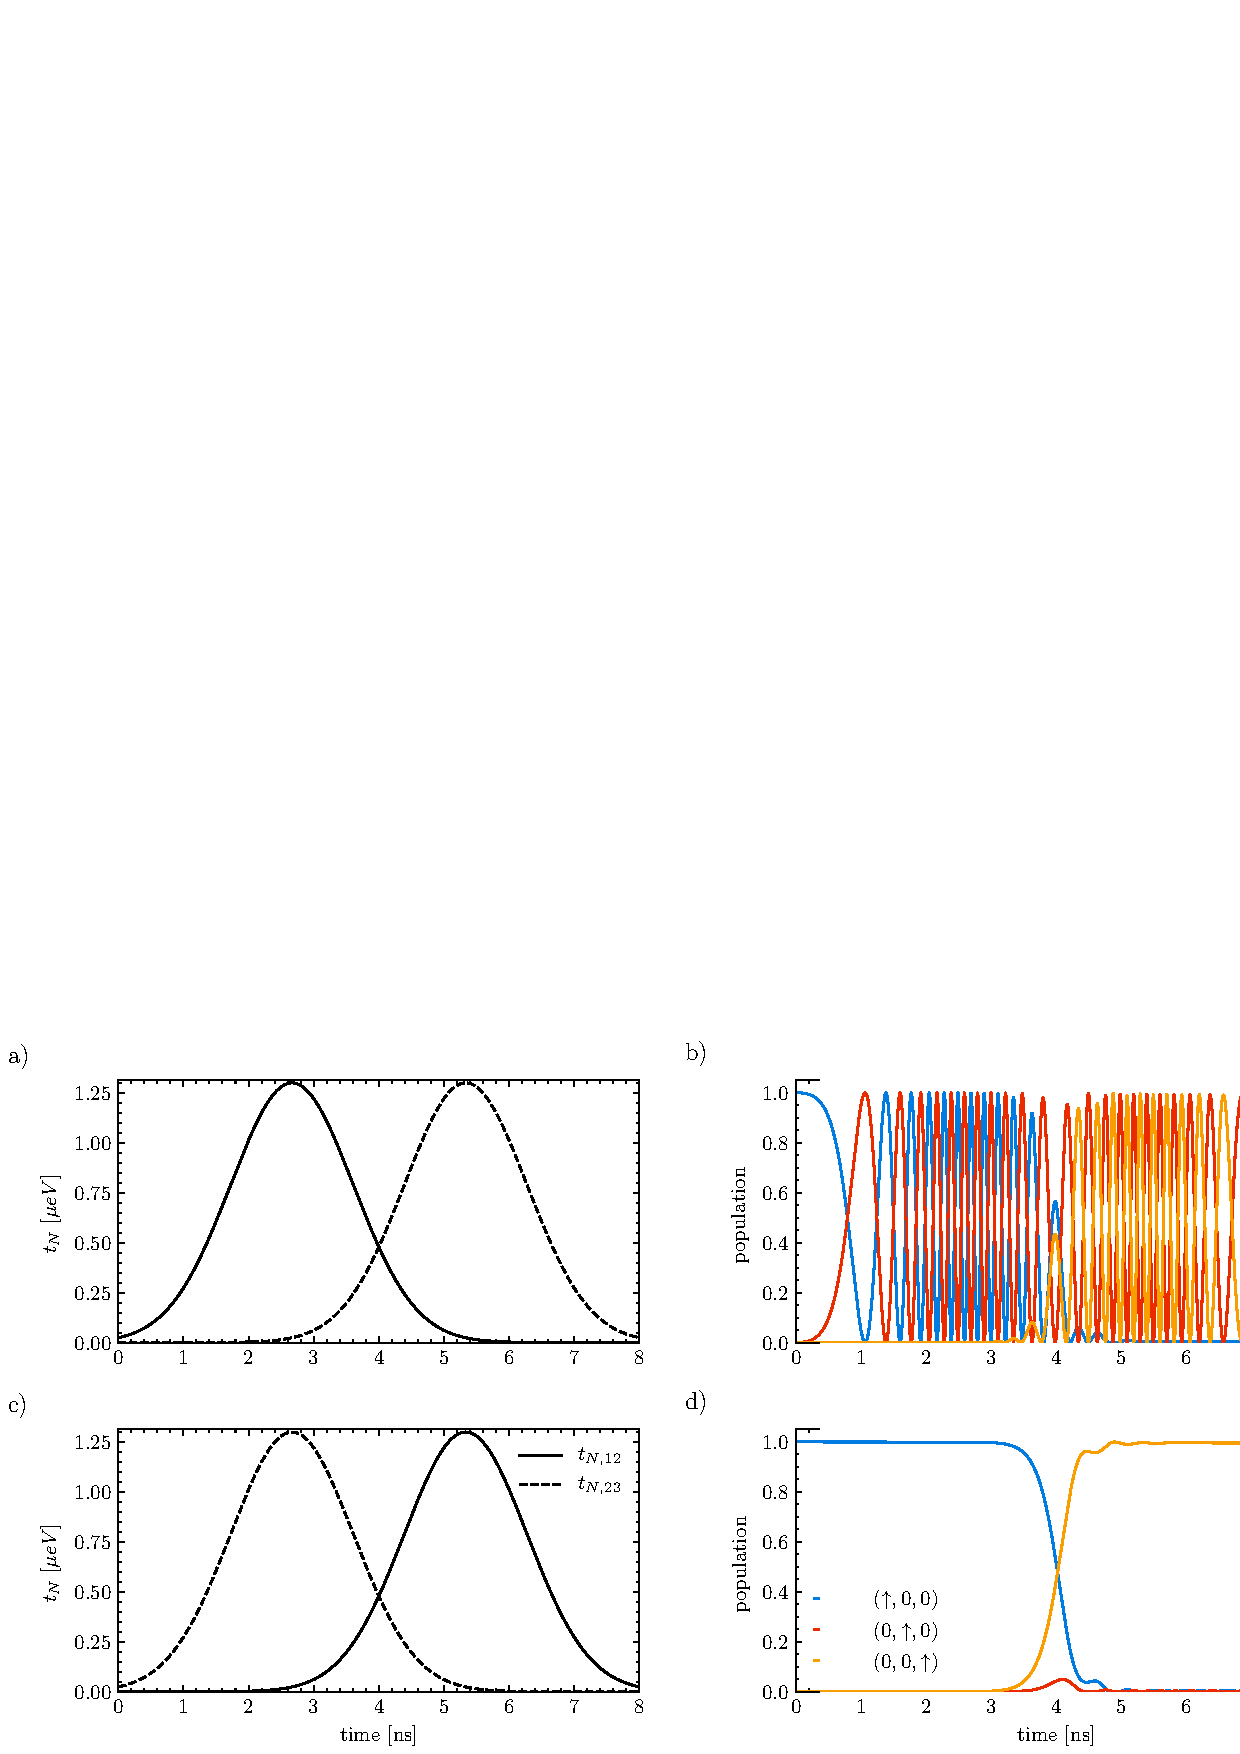
\includegraphics[width=\linewidth]{CTAP_TQD_Results.pdf}
	\caption{Gaussian pulses used for a) intuitive order and c) counter-intuitive order. The spin-flip tunneling rates have the dependence $t_F=0.4\times t_N$. The maximum values for the tunneling rates is $t_0=1.3\; \mu$eV. Evolution of the system for b) intuitive order and d) counter-intuitive order. Both in b) and d) the population of $\ket{0,\uparrow,0}$ (red) and $\ket{0,\downarrow,0}$ (orange) overlap at all times.}
	\label{fig:CTAP_TQD_Results}
\end{figure}

If we want to improve the fidelity we can use longer times or increase the maximum amplitude of the pulses, but let's try something different and check if we can apply CD to this system. As we have seen in Sec.~\ref{sec:CD} the Hamiltonian that we must add corresponds to
\begin{equation}
\hat{\mathcal{H}}_{\text{CD}}=i\hbar\sum_n|\dot{\phi}_n(t)\rangle\bra{\phi_n(t)}\; ,
\label{eq:CD_Hamiltonian}
\end{equation}
where we have assumed that $\bra{\phi_n(t)}\dot{\phi}_n(t)\rangle=0$. Computing analytically the instant eigenvectors we obtain the Hamiltonian

\begin{equation}
\hat{\mathcal{H}}_{\text{CD}}=\hbar\mqty(0 & 0 & 0 & 0 &  0& -\dot{\varphi}\\
0 & 0 &0 & 0 & -\dot{\varphi} & 0\\
0 & 0 &0 & 0 &0  & 0\\
0 & 0 &0 &0 &0 &0\\
0 & -\dot{\varphi} & 0 & 0 & 0 & 0 \\
-\dot{\varphi} & 0 & 0 & 0 & 0 & 0)\; ,
\end{equation}
where we have set the SO phase $\theta=\pi/2$ to simplify the result. The new terms added correspond to a direct coupling between the ends of the array, what is impossible to obtain in a experimental setup. A similar problem was treated in other works \cite{Ban2018} by finding a proper unitary operator such that
\begin{equation}
\tilde{\mathcal{H}}=U^\dagger\hat{\mathcal{H}}U-iU^\dagger \dot{U}=\tilde{t}_{N,12}\hat{c}_1^\dagger\hat{c}_2+\tilde{t}_{N,23}\hat{c}_2^\dagger\hat{c}_3+\text{H.c.}
\end{equation}
The system treated in the mentioned work was populated with electrons instead of holes, so the spin-flip tunneling is not considered and the Hamiltonian is given by a $3\times 3$ matrix. Finding the correct transformation that leads our six levels Hamiltonian with couplings only in the neighbour QDs is extremely challenging, so let's try to apply inverse engineering. The wave function can be parametrized as
\begin{equation}
	\ket{\Psi(t)}=\cos\chi\cos\eta\ket{\uparrow,0,0}+\frac{\sin\eta}{\sqrt{2}}(i\ket{0,\uparrow,0}+\ket{0,\downarrow,0})+i\sin\chi\cos\eta \ket{0,0,\downarrow}\; ,
	\label{eq:wave_functions_parametrization}
\end{equation} 
what is very similar to the parametrization used in a fast long-transfer for electrons in a triple quantum dot \cite{Ban2018}. The two auxiliary parameters that we can introduced are time dependent functions, using Eq.~(\ref{eq:wave_functions_parametrization}) in the time-dependent Schrödinger equation we obtain a system of equations given by
\begin{subequations}
	\begin{gather}
	-\frac{t_{N,12}\sin\eta}{\sqrt{2}}(1+ie^{i\theta})=0\; ,\\
	-\frac{t_{N,12}\sin\eta}{\sqrt{2}}(i+e^{i\theta})=-i(\dot{\eta}\cos\chi\cos\eta+\dot{\chi}\cos\eta\sin\chi)\; ,\\
	\frac{\dot{\eta}\cos\eta}{\sqrt{2}}=t_{N,12}\cos\eta\cos\chi+ie^{i\theta}t_{N,23}\cos\eta\sin\chi\; ,
	\end{gather}
\end{subequations}
where we have only written down the independent equations. The first equation is only verified, apart from the trivial $\eta=0$, if the phase $\theta=\pi/2$, what corresponds the situation in which only the Dresselhaus SOC is present. Using this the solution for the auxiliary parameters are
\begin{subequations}
	\begin{align}
		\dot{\eta}&=\sqrt{2}(t_{N,12}\cos\chi-t_{N,23}\sin\chi)\; ,\\
		\dot{\chi}&=\sqrt{2}\tan\eta(t_{N,12}\sin\chi+t_{N,23}\cos\chi)\; .
	\end{align}
\end{subequations}
This can be easily inverted obtaining the equations for the tunneling rates
\begin{subequations}
	\begin{align}
	t_{N,12}&=(\dot{\eta}\cos\chi+ \dot{\chi}\sin\chi\cot\eta)/\sqrt{2}\; ,\\
	t_{N,23}&=(-\dot{\eta}\sin\chi+ \dot{\chi}\cos\chi\cot\eta)/\sqrt{2}\; .
	\end{align}
	\label{eq:STA_pulses}
\end{subequations}
Our initial state is $\ket{\Psi(t=0)}=\ket{\uparrow,0,0}$ and the target final state is $\ket{\Psi(t=t_f)}=\ket{0,0,\downarrow}$ up to a phase. The boundary conditions in then set to $\chi(t=0)=\eta(t=0)=\eta(t=t_f)=0$ plus $\chi(t=t_f)=\pi/2$. More conditions can be imposed in order to obtain smooth pulses $\dot{\chi}(t=0)=\dot{\chi}(t=t_f)=\ddot{\chi}(t=0)=\ddot{\chi}(t=t_f)=\dot{\eta}(t=0)=\dot{\eta}(t=t_f)=0$. One of many different ansatz that verify the boundary conditions is
\begin{subequations}
	\begin{align}
	\chi&=\frac{\pi t}{2 t_{f}}-\frac{1}{3} \sin \left(\frac{2 \pi t}{t_{f}}\right)+\frac{1}{24} \sin \left(\frac{4 \pi t}{t_{f}}\right)\; , \\
	\eta&=\arctan \left(\dot{\chi} / \alpha_{0}\right)\; ,
	\end{align}
\end{subequations}
where $\alpha_0$ is an arbitrary parameter with units of frequency. The population in the middle dot $P_2(t)\equiv \sin^2\eta$ presents a maximum at $t=t_f/2$ given by
\begin{equation}
	P_2(t=t_f/2)=\frac{16\pi^2}{16\pi^2+(3\alpha_0t_f)^2}\; .
	\label{eq:population_middle}
\end{equation}
Here we can see that we have two possibilities to decrease the population in the middle dot. One of them is to increase the total time, so the transfer is more adiabatic-like following the dark state. If we want to keep lower operation times we can also increase the value of the parameter $\alpha_0$, at the expense of obtaining higher values for the pulses, thus consuming more energy in the protocol. Higher energy consumption leads to higher heat dissipation losses in the experimental equipment and the sample may reach too high temperatures. Therefore, we will have to make a compromise between short operating times, not too high pulses and sufficiently low mid-point populations. In Fig.~\ref{fig:STA_TQD_Results_1} we show the results for the pulses and the evolution of the system. The total time is set to $t_f=10$ ns and $\alpha_0=5$, using this in Eq.~(\ref{eq:population_middle}) we obtain a maximum population in the middle dot of 0.7\%, what is the exactly the same value than the one obtained in the simulation. The error in the fidelity $\epsilon\equiv 1-\mathcal{F}$ with this parameters is extremely low $\epsilon\sim 10^{-11}$.
\begin{figure}[!htb]
	\centering
	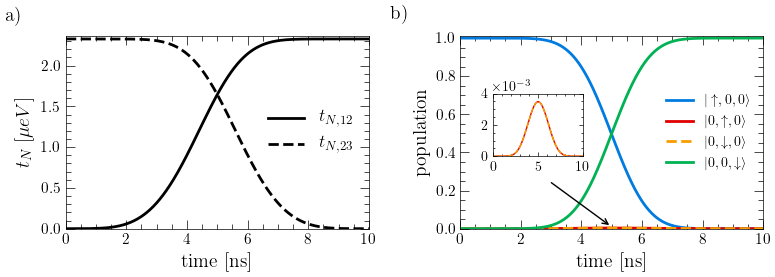
\includegraphics[width=\linewidth]{STA_TQD_Results_1.pdf}
	\caption{a) Pulses and b) evolution obtained for the inverse engineering protocol. The spin-flip tunneling rates are equal to the spin-conserving ones $t_{F,ij}=t_{N,ij}$, with a phase $\theta=\pi/2$. The simulation is done with the parameter $\alpha=5$. The population of $\ket{0,\uparrow,0}$ (red) and $\ket{0,\downarrow,0}$ (orange) overlap at all times.}
	\label{fig:STA_TQD_Results_1}
\end{figure}

This results corresponds to the ideal case, in which all the parameters are set with perfect control. But this is not usually the case when trying to implement the protocol in a experimental setup. The existence of the dark state is conditioned to the dots being in resonance $\varepsilon_i=0$ with $i=1,2,3$ denoting each dot. But this is difficult to achieved, and a non zero detuning can appear between dots. The dependence of the error in the fidelity varying the parameters $\varepsilon_{2}$ and $\Delta\varepsilon_{31}\equiv \varepsilon_3-\varepsilon_1$ is shown in Fig.~\ref{fig:STA_TQD_Combined_SF} a). Here we present the absolute value of the decimal logarithm, so colors closer to red means higher fidelities, e.g. $\abs{\log_{10}(\epsilon)}=4\rightarrow\mathcal{F}=0.9999$. In this figure we can observe that the protocol is more sensitive to the detuning of the lateral dots than to the central dot. Other source of error is the ration between the tunneling rates $t_{F,ij}=xt_{N,ij}$, which must we set to $x=1$ as we have seen above. The same occur to the SO phase what is set to $\theta=\pi/2$. The result for the error in the fidelity in terms of how much these two parameters deviate from their respective ideal values is shown in Fig.~\ref{fig:STA_TQD_Combined_SF} b). The transfer is almost insensitive to an error in the phase up to $\theta=\pi/2\pm\pi/4$, from this point the fidelity drops rapidly to $\mathcal{F}=0.25$ when $\theta=0$ of $\theta=\pi$. At this point the final result is a coherent mixture of the hole in both edges and spines with a probability of $25\%$ for each state. The dependence with the ratio has the opposite behaviour, near $x\rightarrow 0$ the sensitive is high, while as we move away from this value the fidelity acquired a more constant behaviour decreasing the sensitivity.

\begin{figure}[!htb]
	\centering
	\includegraphics[width=\linewidth]{STA_TQD_Combined_SF.pdf}
	\caption{Colour plot with overlayed contour showing the error in the fidelity $\epsilon\equiv 1-\mathcal{F}$ for the IE protocol applied to the long transfer of a HH in a TQD with spin flip. a) Variations in the detuning of the dots, with $\varepsilon_{31}\equiv \varepsilon_3-\varepsilon_1$, b) variations in the ration $t_{F,ij}=xt_{N,ij}$ and the SO phase $\theta$. In both figures the shapes at the top and at the right of the colour map represents the cross sections passing thought the middle of the y-axis and x-axis respectively. Note the absolute value, higher fidelities, i.e. lower errors, are represented with colors closer to red.}
	\label{fig:STA_TQD_Combined_SF}
\end{figure}

Other possibility of error in the protocol is the existence of dephasing mechanisms. We are considering a solid-state system, so we ignore $T_1$ rates, as $T_2$ is generally much faster. The equation that represent the dynamics of the system is given by Eq.~(\ref{eq:dephasing_ME})
\begin{equation}
	\frac{d}{dt}\rho=-\frac{i}{\hbar}[\hat{\mathcal{H}},\rho]-\frac{\gamma}{2}(\rho-\operatorname{diag}(\rho))\; ,
\end{equation}
where we have assumed that the pure dephase acts equally on all coherences. We can expect that for higher values of $T_2$, i.e. lower values of the coupling $\gamma$, the fidelity increases with time. However the dephasing is accumulated over time, so for high enough coupling with the environment the fidelity will reach a peak at certain time and then continuously decrease. In Fig.~\ref{fig:CTAP_vs_STA} we present the results for the fidelity as a function of the total pulse time and dephasing $\gamma$. In this figure we can observe the advantage of the STA scheme compared to CTAP. Inverse engineering is more robust to dephasing. This is because the CTAP protocol takes longer times to achieve high fidelities compared to the IE scheme. To compare both protocols under equal conditions we have matched the maximum values for each pulses. 
\begin{figure}[!htb]
	\centering
	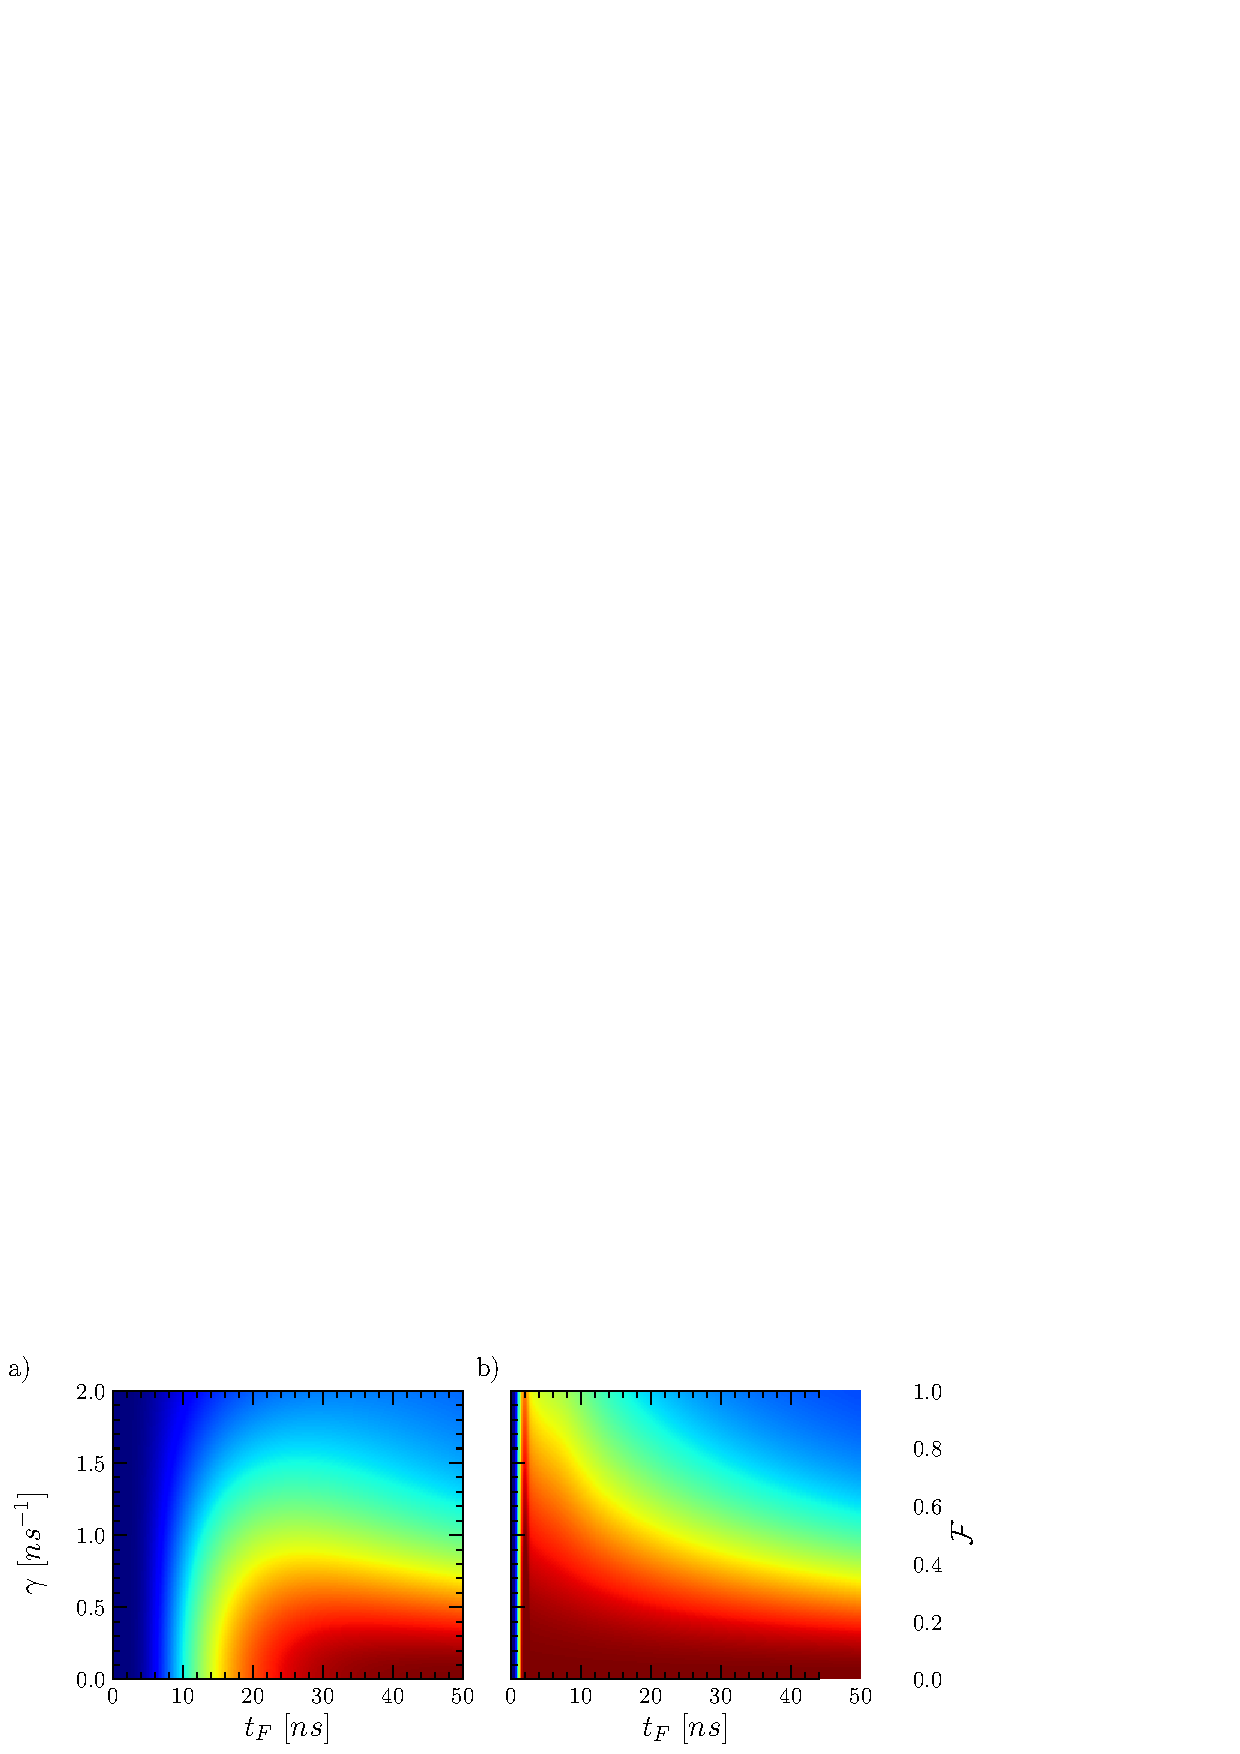
\includegraphics[width=\linewidth]{CTAP_vs_STA.pdf}
	\caption{Colour plot showing the fidelity for the a) CTAP protocol and b) IE scheme. The maximum value for the Gaussian shapes in a) is set to $t_0=2.3\; \mu$eV. For b) the STA pulses we have used the parameter $\alpha_0=5$ ns$^{-1}$. Both figures shares y-axis and the colour bar.}
	\label{fig:CTAP_vs_STA}
\end{figure}

\section{Long range transference conserving spin}
Let us go back to the equation of the dark state, Eq.~(\ref{eq:dark_state}). We have considered the case of a long range transfer changing the spin of the particles, but is we set the SO phase to $\theta=0$ or $\theta=\pi$ we have the opposite, where the transfer conserve the spin. The dark state is then written as
\begin{equation}
	\ket{\phi_{\text{DS},1}}=-\cos(\varphi)\ket{\downarrow,0,0}+\sin(\varphi)\ket{0,0,\downarrow}\; ,
\end{equation}
where we have defined the angle $\tan(\varphi)\equiv t_{N,12}/t_{N,23}$, as in the previous section. Here we are working with the transfer of a spin down particle, but the same is valid for the spin up case. The CTAP protocol give us results almost identical to the spin flip long range transfer, so we are not going to repeat them. For the CD protocol we can use one more time Eq.~(\ref{eq:CD_Hamiltonian}) to obtain the counter term that we must add, which is written as
\begin{equation}
	\hat{\mathcal{H}}_{\text{CD}}=\hbar \mqty(0 & 0 & 0 &0 &i\dot{\varphi} & 0 \\ 0 & 0 & 0 & 0 & 0 & i\dot{\varphi}\\ 0 & 0 & 0 & 0 & 0 & 0 \\ 0 & 0 & 0 & 0 & 0 & 0 \\ -i\dot{\varphi} & 0 & 0 & 0 & 0 & 0 \\ 0 & -i\dot{\varphi} & 0 & 0 & 0 & 0)\; .
\end{equation}
As expected the new term that we must add in order to achieve a perfect adiabatic transition pass thought coupling second neighbour QD's, what can be extremely challenging. One more time finding a correct unitary transformation to recover the total Hamiltonian is something more feasible is highly non trivial, and we have not being able to obtain it. So lets move to IE, where we parametrize the wave functions in a similar way than before
\begin{equation}
\ket{\Psi(t)}=e^{i\alpha}\cos\chi\cos\eta\ket{\downarrow,0,0}+e^{i\beta}\frac{\sin\eta}{\sqrt{2}}(x\ket{0,\uparrow,0}+\ket{0,\downarrow,0})+e^{i\delta}\sin\chi\cos\eta \ket{0,0,\downarrow}\; ,
\label{eq:wave_functions_parametrization_2}
\end{equation} 
where we have some phases $\alpha,\beta,\delta$ that must be fixed by the Schrödinger equation. But when we try to introduce the wave function in this equation we obtain two conditions that can not be solved simultaneously, no matter the values for the phases that we have introduced
\begin{equation}
	\begin{split}
	ixe^{i\beta}\cos(\eta)\dot{\eta}&=e^{i\alpha}t_{N,12}x\cos(\eta)\cos(\chi)+e^{i\delta}t_{N,23} x\cos(\eta)\sin(\chi))\; ,\\
	ie^{i\beta}x\cos(\eta)\dot{\eta}&=-e^{i\alpha}t_{N,12}\cos(\eta)\cos(\chi)-e^{i\delta}t_{N,23} \cos(\eta)\sin(\chi))\; .
	\end{split}
\end{equation}
This is an indication that we should propose a more complex parametrization than the one shown here. But is difficult to think in a more general way of written the solution without overcomplicate the problem. However, the dark state is almost identical to what we have previously seen, so let us use the pulses obtained in Eq.~(\ref{eq:STA_pulses}), now with $x\neq 1$ and $\theta=0$. the result are shown in Fig.~\ref{fig:STA_TQD_Results_2} b). From here we can conclude that, even in the pulses was designed for this specific case, the transfer is achieved with low error $\mathcal{\epsilon}\sim 10^{-9}$ and with a moderate population in the middle dot. A difference with the spin-flip long range transfer is the population of $\ket{\uparrow,0,0}$ and $\ket{0,0,\uparrow}$, whose maximum value reach $2\times10^{-4}$. As one would expect, the maximum population in the central dot is no longer given by Eq.~(\ref{eq:population_middle}) that predict a value of $0.7\%$, however the value obtained in the simulations reaches $2.6\%$.
\begin{figure}[!htb]
	\centering
	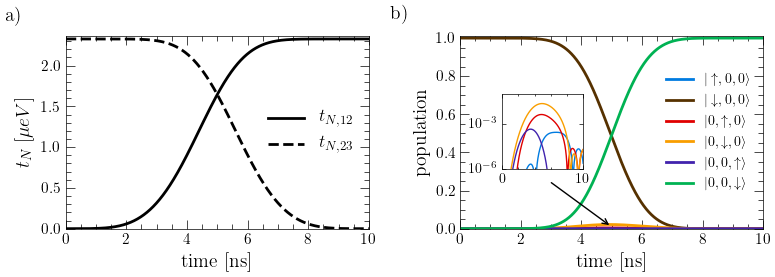
\includegraphics[width=0.9\linewidth]{STA_TQD_Results_2.pdf}
	\caption{a) Pulses and b) evolution obtained for the inverse engineering protocol. The spin-flip tunneling rates are equal to the spin-conserving ones $t_{F,ij}=0.4\times t_{N,ij}$, with a phase $\theta=0$. The simulation is done with the parameter $\alpha=5$.}
	\label{fig:STA_TQD_Results_2}
\end{figure}

